\documentclass[tikz,border=2pt]{standalone}
\usepackage{amsmath,amssymb}
\usepackage{pgfplots}
\pgfplotsset{compat=1.18}
\usetikzlibrary{arrows.meta}
\begin{document}
% 10-year endowment insurance at delta = 0.03: Z = v^{min(T_x,10)} = e^{-0.03 min(T_x,10)} is e^{-0.03T_x}
% for death before 10 and e^{-0.3} ~ 0.741 on survival; at lambda = 0.02 its mean is E[Z] ~ 0.764.
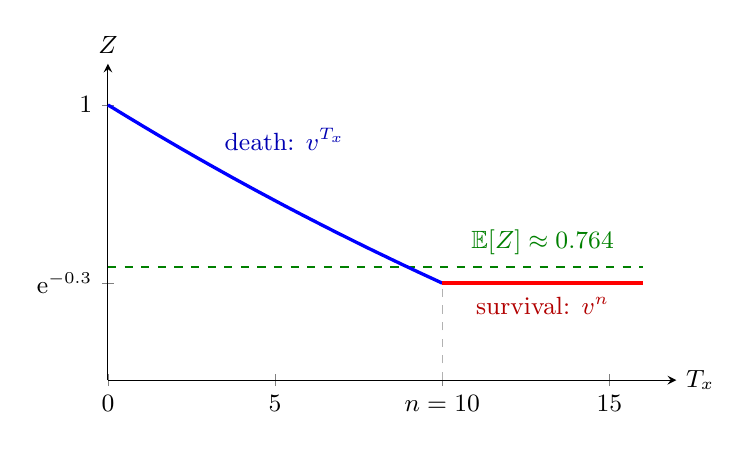
\begin{tikzpicture}[font=\small, >={Latex[length=2mm]}]
  \begin{axis}[
    axis lines=left, xmin=0, xmax=17, ymin=0.6, ymax=1.06,
    xtick={0,5,10,15}, xticklabels={$0$,$5$,$n=10$,$15$},
    ytick={0.7408,1}, yticklabels={$\mathrm{e}^{-0.3}$,$1$},
    xlabel={$T_x$}, ylabel={$Z$},
    xlabel style={at={(axis description cs:1,0)}, anchor=west},
    ylabel style={rotate=-90, at={(axis description cs:0,1)}, anchor=south},
    samples=60, width=8.8cm, height=5.6cm, clip=false]
    \draw[gray!60, thin, dashed] (axis cs:10,0.6) -- (axis cs:10,0.7408);
    \draw[green!50!black, thick, dashed] (axis cs:0,0.7639) -- (axis cs:16,0.7639);
    \addplot[blue, very thick, domain=0:10] {exp(-0.03*x)};
    \addplot[red, very thick, domain=10:16] {exp(-0.3)};
    \node[blue!70!black, anchor=south west] at (axis cs:3.2,0.92) {death: $v^{T_x}$};
    \node[red!70!black, anchor=north] at (axis cs:13,0.735) {survival: $v^{n}$};
    \node[green!50!black, anchor=south] at (axis cs:13,0.768) {$\mathbb{E}[Z]\approx0.764$};
  \end{axis}
\end{tikzpicture}
\end{document}
